\section{Background}
\subsection{Observations in Optical Astronomy}
\subsubsection{Telescope Optics}
In our observation we used a \SI{50}{\cm} reflector telescope of the Cassagrain type which is available in AIFA. 
% The incident light from a source first falls on a concave parabolic primary mirror (1) then re-reflected by a hyperbolic convex mirror (2). The rear focus (A) of the secondary is placed in the focus of the primary mirror such that the light is collimated in the convex focus of the secondary mirror (B) via an small hole, which is making without disturbing the focal length of such mirror, in the primary mirror. A detector is placed behind the primary mirror because light rays are collimated at (B).
A schematic diagram of this telescope is as shown in Fig. \ref{Fig:telescope}.
\begin{figure}[H]
	\centering
	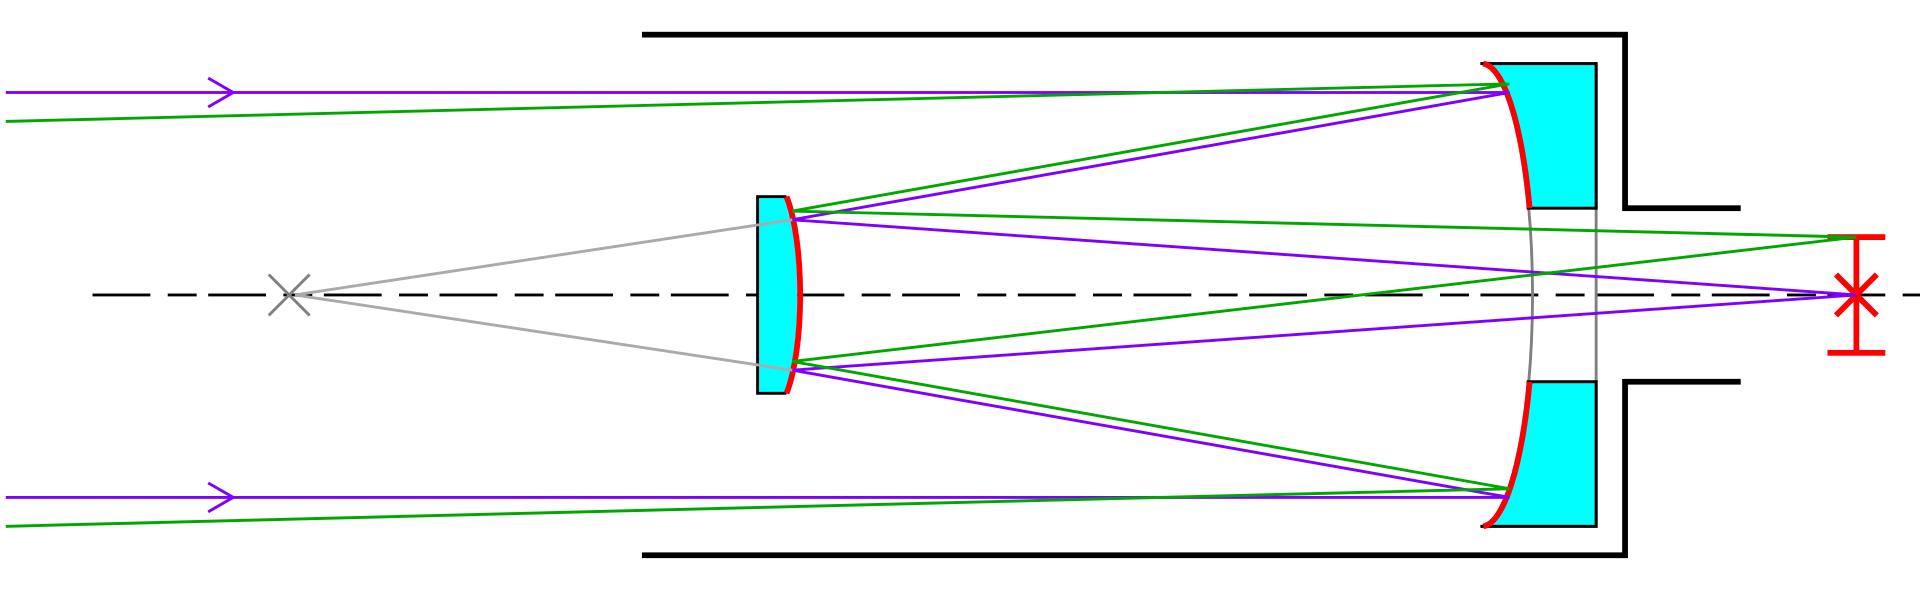
\includegraphics[width=0.6\linewidth]{lens.png}
	\caption{Schematic light path in a Cassegrain telescope\cite{manual}.}%
	\label{Fig:telescope}	
\end{figure}

% The spatial resolution is given by the Rayleigh criterion,
% \begin{eqnarray}
% \Delta\theta = 1.22 \frac{\lambda}{\text{D}}
% \end{eqnarray}
% \noindent
% where, \text{D} is the primary aperture and $ \lambda $ is the wavelength of light rays. The actual resolution is always very less for ground based telescope due to the numerous effect of Earth's atmosphere. \\
%

% \subsubsection{Seeing and Airmass}
% The earth's atmosphere has considered as a part of the optical system for ground based astronomical observation. So, numerous effect are arises, mostly, turbulence in the atmosphere leads fluctuation on refractive index on short spatial and temporal scale. This result in a blurring and scintillation of the PSF. That complicated shape can be represented by approximately Gaussian shape in two dimensions. Thus, the full width at half maximum(FWHM) size of the Gaussian shape of such stellar image is called Seeing of the image. It helps to measure the actual resolution in a particular observation. For Bonn, a seeing is 2 arcsec is a best value.\\
%
% The column density on the atmosphere through which the light travels compared to vertical in-fall is called Airmass. For an angular distance z from zenith the best approximation can be computed as,
% \begin{equation}
	% a=\frac{1}{\cos z}
% \end{equation}
% Where, $ a=1 $ for an object at the zenith i.e. $ z= 0^{\circ} $ and $ a=\infty $ at horizon.
% Thus, the best possible observing position is near the zenith.\\

\subsubsection{Magnitude}
In optical astronomy, the optical brightness of a source is called magnitude.

The difference in magnitudes between two sources is defined on the basis of ratio of their observed fluxes $ {S}_{1} $ and $ {S}_{2} $ as,
\begin{equation}
	\Delta {m}= {m}_{1}-{m}_{2}=-(100^{1/5}) \cdot \log_{10} \bigg(\frac{{S}_{1}}{{S}_{2}}\bigg)
\end{equation}
With this definition, fainter sources have higher magnitude.

\subsubsection{Coordinate system}
There are different co-ordinate systems 
% (like as equatorial co-ordinate system, galactic co-ordinate system, and etc.)
use to quantify the position of celestial objects in optical astronomy. The equatorial system is a most common system for identifying and cataloging the sources. In this system the framework of terrestrial latitude and longitude projected from the centre of earth onto the sky~\cite{manual}.
\begin{itemize}
	\item Declaration is an analogy to latitude in geography. Here, the north pole having declination of $ \delta=90^{\circ} $ and projection of south pole is  $ \delta= -90^{\circ} $. It is express as degree, minute and second. 
	\item Right Ascension, $\alpha $, is equivalent to longitude with the equatorial zero point. It is express as hour, minute and second.
\end{itemize}

\subsection{Charge-coupled device}
Charge-coupled device (CCD) is a two-dimensional detector used to detect electromagnetic radiations. It responds to wide wavelength range (from near infrared to the soft X-ray). Its working principle relies on photoelectric effects, thus usually highly linear~\cite{manual}.

% The distribution of photons is converted to a distribution of charge packets which are collected and stored in three dimensional potential wells. To measure the amount of charge in each packets they have to be transported across the full detector surface to output amplifier. During this transportation of charge packets potential barriers in the transport direction can be manipulated by applying appropriate voltage waveform. The transport is done by parallel shift and series shift. On this functioning principle electrons are shifted, detected and converted in a digital number or count or analog-to-digit unit (ADU) at a rate of about 30 kHz.

Good quality CCDs are supposed to have high quantum efficiency, low read noise, and excellent linearity. In this experiment we will determine these properties. Some of these properties are discussed below.

\subsubsection{Stability}
There are several aspect to hold excellent stability characteristic by a CCD. Some of them are
\begin{itemize}
	\item CCD is geometrically very stable because it is contracted by pure silicon.
	\item It keeps its performance over years without degradation.
	\item It has very high sensitivity; however, very insensitive to over-exposure.
\end{itemize}

\subsubsection{Dark Current}
Dark current is essentially thermal noise. It depends on the temperature of CCD. At room temperature, it fills CCD pixels to their saturation level within a short period of time (a minute or even less). Therefore, it is necessary to keeps the detector system at a low temperature. The cooling of CCD is done thermo-electrically with closed cycle system or by using liquid nitrogen~\cite{manual}.

The dark current $ {I}_{\text{dark}} $ changes  with temperature  $T$ as
\begin{equation}
{I}_{\text{dark}}=c {T}^{3/2} e^{-{\frac{{E}_{{g}}}{2k_{\text{B}}{T}}}}
\label{Equ:DarkCurrent}
\end{equation}
where $ {E}_{{g}}= \SI{1.16}{\eV} $ is the silicon band gap energy, $ k_{\text{B}}=\SI{8.62e-5 }{\eV\per\kelvin}$ is the Boltzmann constant, and $ c $ is a detector specific constant. In this report, dark current is always given in unit of \si{\ele\per\px\per\s}, i.e.~before A/D conversion.

\subsubsection{Gain}
The ratio between the amount of charge in a CCD pixel and the corresponding digital number after A/D conversion is called detector gain $k$~\cite{manual}. It is measured in the unit of $ e^{-}/\si{ADU} $. It can be calculation on the basis of the assumption that photon detector is Poisson distributed~\cite{manual}.
\begin{equation}
	{N}_{e}= \sigma^2_{e}= k{N}_{e, {d}}= k^2 {\sigma}^2_{e,{d}}
\end{equation}
where ${N}_{e}$ and $ \sigma_{e} $ are average number of electron and its standard deviation. Subscript $\text{d}$ means that the numbers are converted to \si{\ADU} already. Therefore, the gain can be determined with
\begin{equation}
k=\frac{{N}_{e, {d}}}{\sigma^2_{e,{d}}}
\label{math:gain}
\end{equation} 

\subsubsection{Quantum Efficiency}
Quantum efficiency is defined as the ratio of produced electrons to the number of photons hitting the detector surface~\cite{manual}. Top order CCDs have the significant wavelength range more than 90$\% $.

\subsubsection{Read-Out Noise}
Even fully covered CCD still have signals varying from pixel to pixel due to the amplification noise occurring in the electronics. The standard deviation of this scatter is called read out noise~\cite{manual}. 

\subsubsection{Noise}
In our detector system there are three sources of noise: read-out noise, photon noise and PRNU noise. The so-called pixel response non-uniformity (PRNU) noise is pixel to pixel variation caused by difference quantum efficiency. Thus the total noise is given by~\cite{manual}
\begin{equation}
	\sigma_{\text{tot}}=\sqrt{ \sigma^2_{\text{RON}} + \sigma^2_{e} + \sigma^2_\text{PRNU}}
\end{equation}
where $ \sigma_{\text{PRNU}} $ is proportional to signal level,
\begin{equation}
\sigma_{\text{PRNU}}={N}_{e} {f}_{\text{PRNU}}
\label{math:fPRNU}
\end{equation} 
$ {f}_{\text{PRNU}} $ is a detector dependent characteristic PRNU factor. It is typically in the order of 0.01~\cite{manual}.

\subsubsection{Linearity and full-well capacity}
One the most appealing feature of CCD as astronomical detectors is it linearity. Here, the output signal is proportional to the incoming photons received by the detector. They are linear over the full dynamic range of $10^4 $ to $10^5 $ and deviation from linearity is just $\pm 0.5 \%$  for well behaved system~\cite{manual}.

The CCD pixels have limited charge capacity. The maximal number of the electrons fitting into a single pixel is called full-well capacity. If one pixel site gets full, electrons will start to spill over to adjacent pixels, causing the so-called  blooming effect~\cite{manual}. Saturation level is essentially the same thing as full-well capacity, but given in the unit of \si{\ADU}.  
